\newpage
\section{Anhang}
  \subsection{Darstellung einiger gängiger WOK}
    \begin{figure}[h!]
      \begin{center}
		    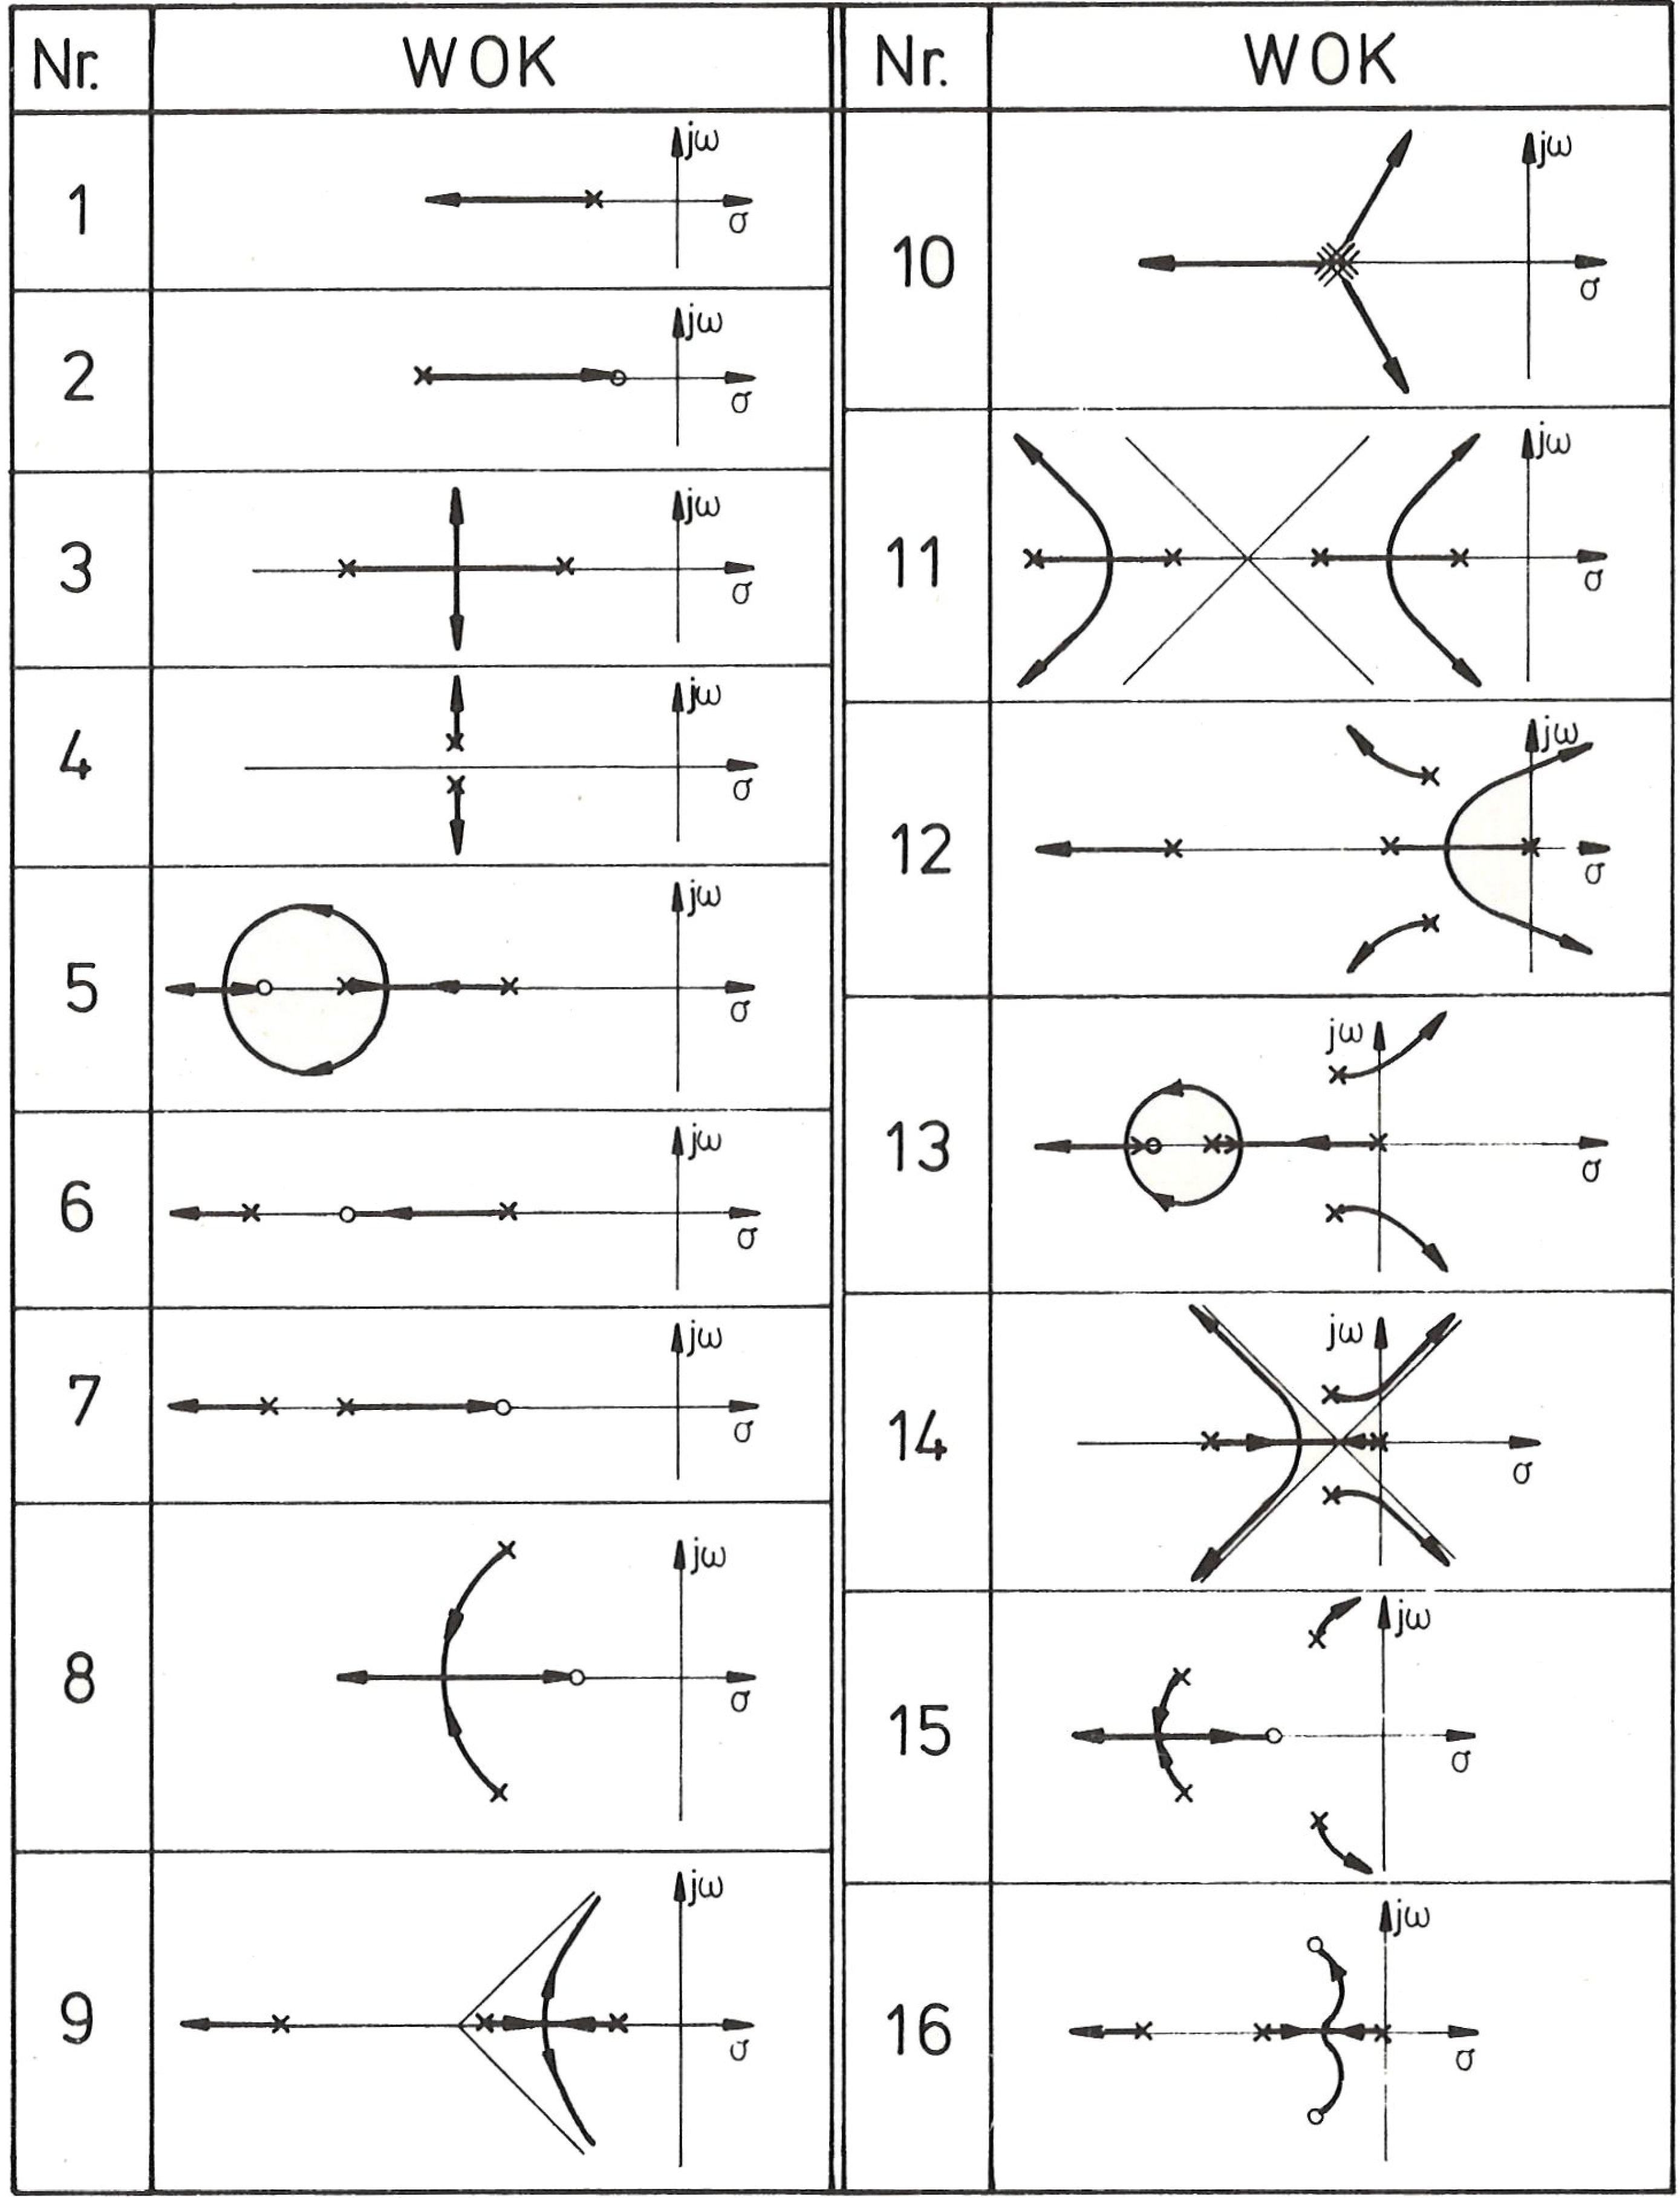
\includegraphics[width=14cm]{./images/BilderWOK.png}
		    \caption{WOK zu einigen geläufigen Pol-/Nullstellenverteilungen, Quelle}
      \end{center}
	  \end{figure}
     \clearpage
 
  \subsection{Bode Approximation}
    \begin{center}
      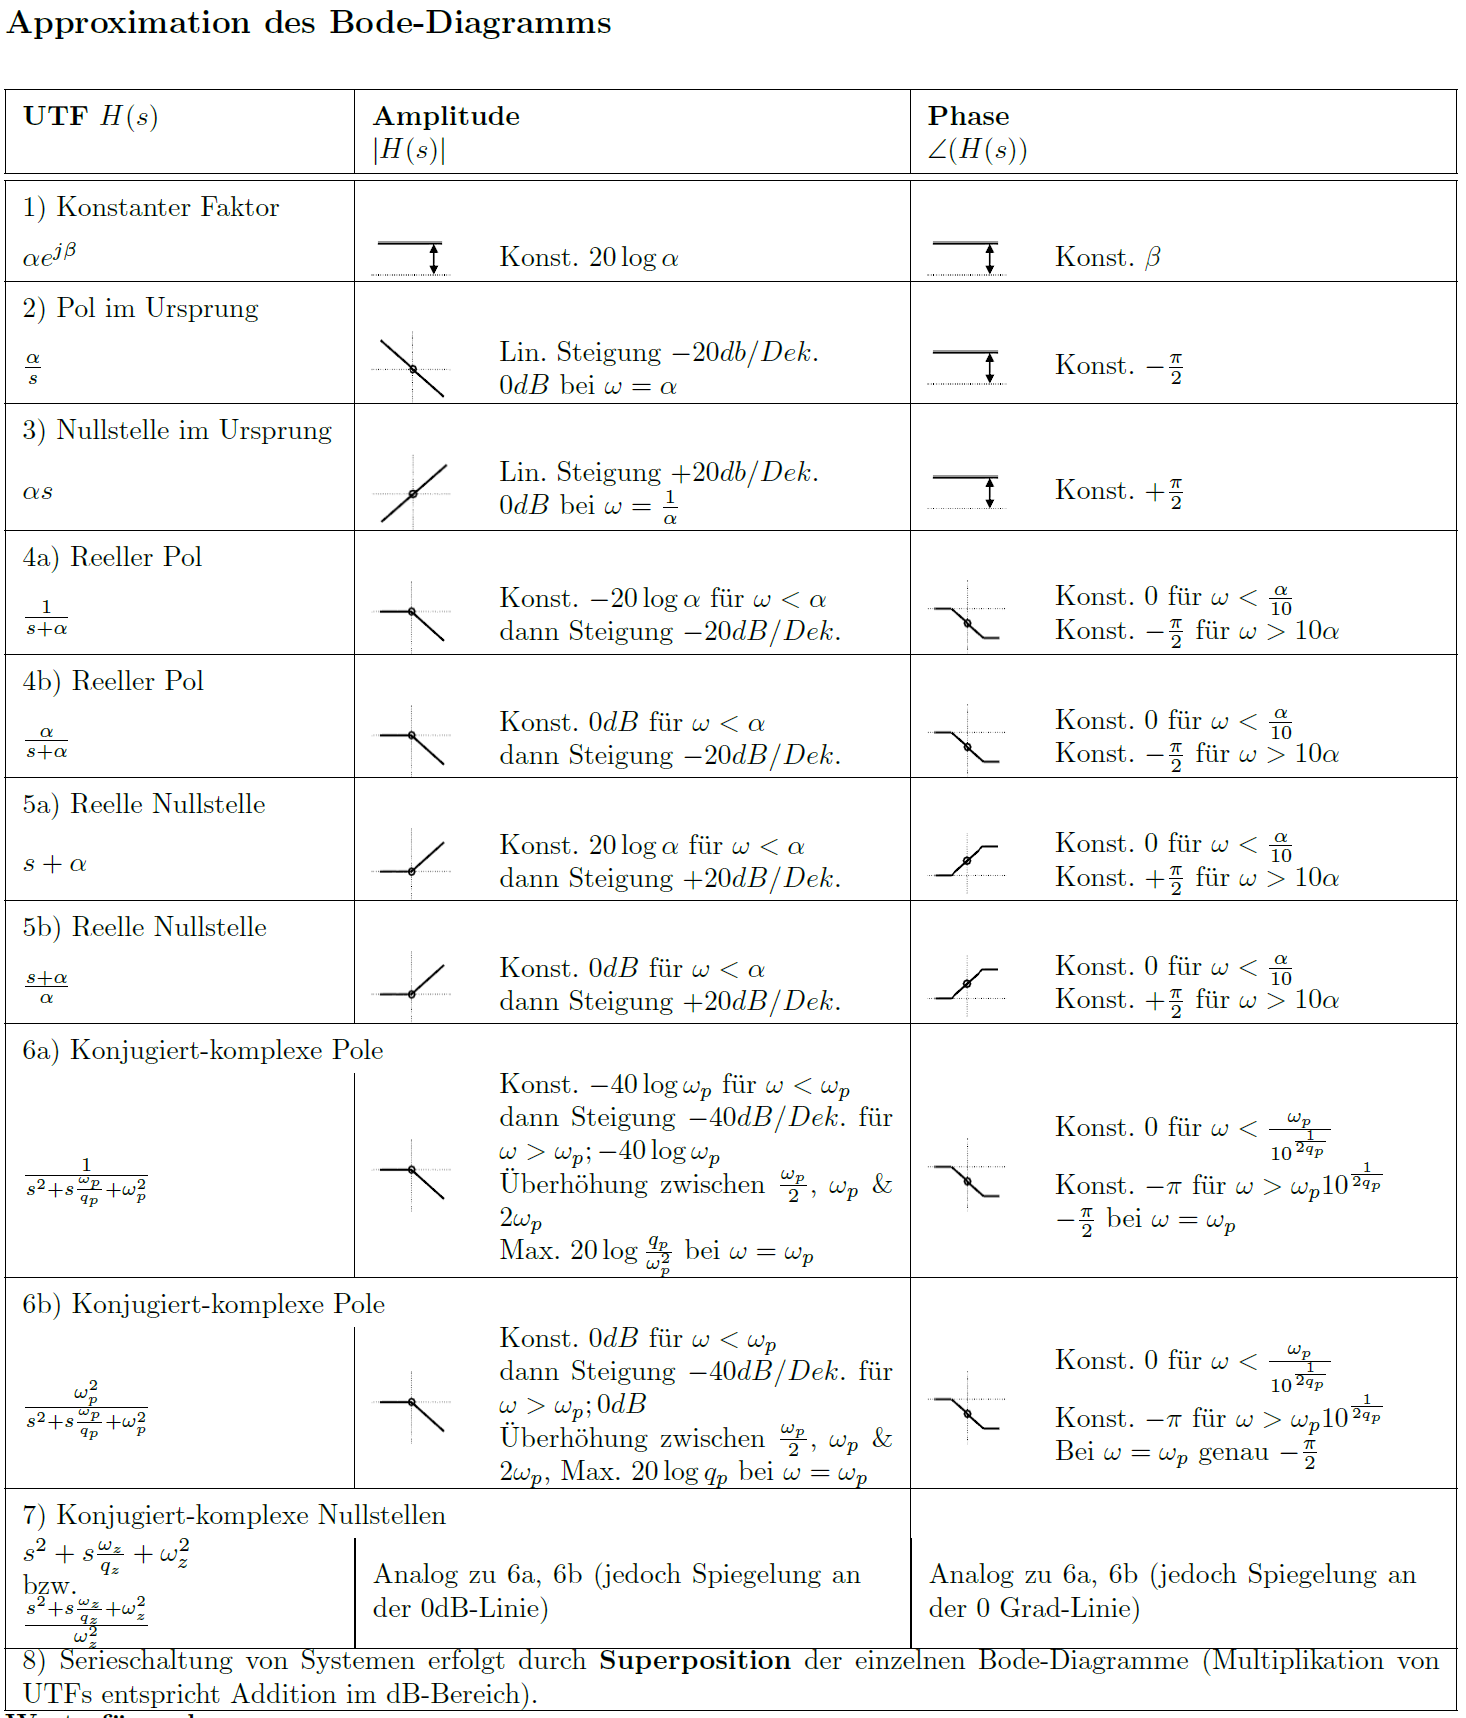
\includegraphics[width=16cm]{./images/BodeAproximationen.png}
    \end{center} 
  
  \subsection{LTI Grundglieder}
  \begin{center}
      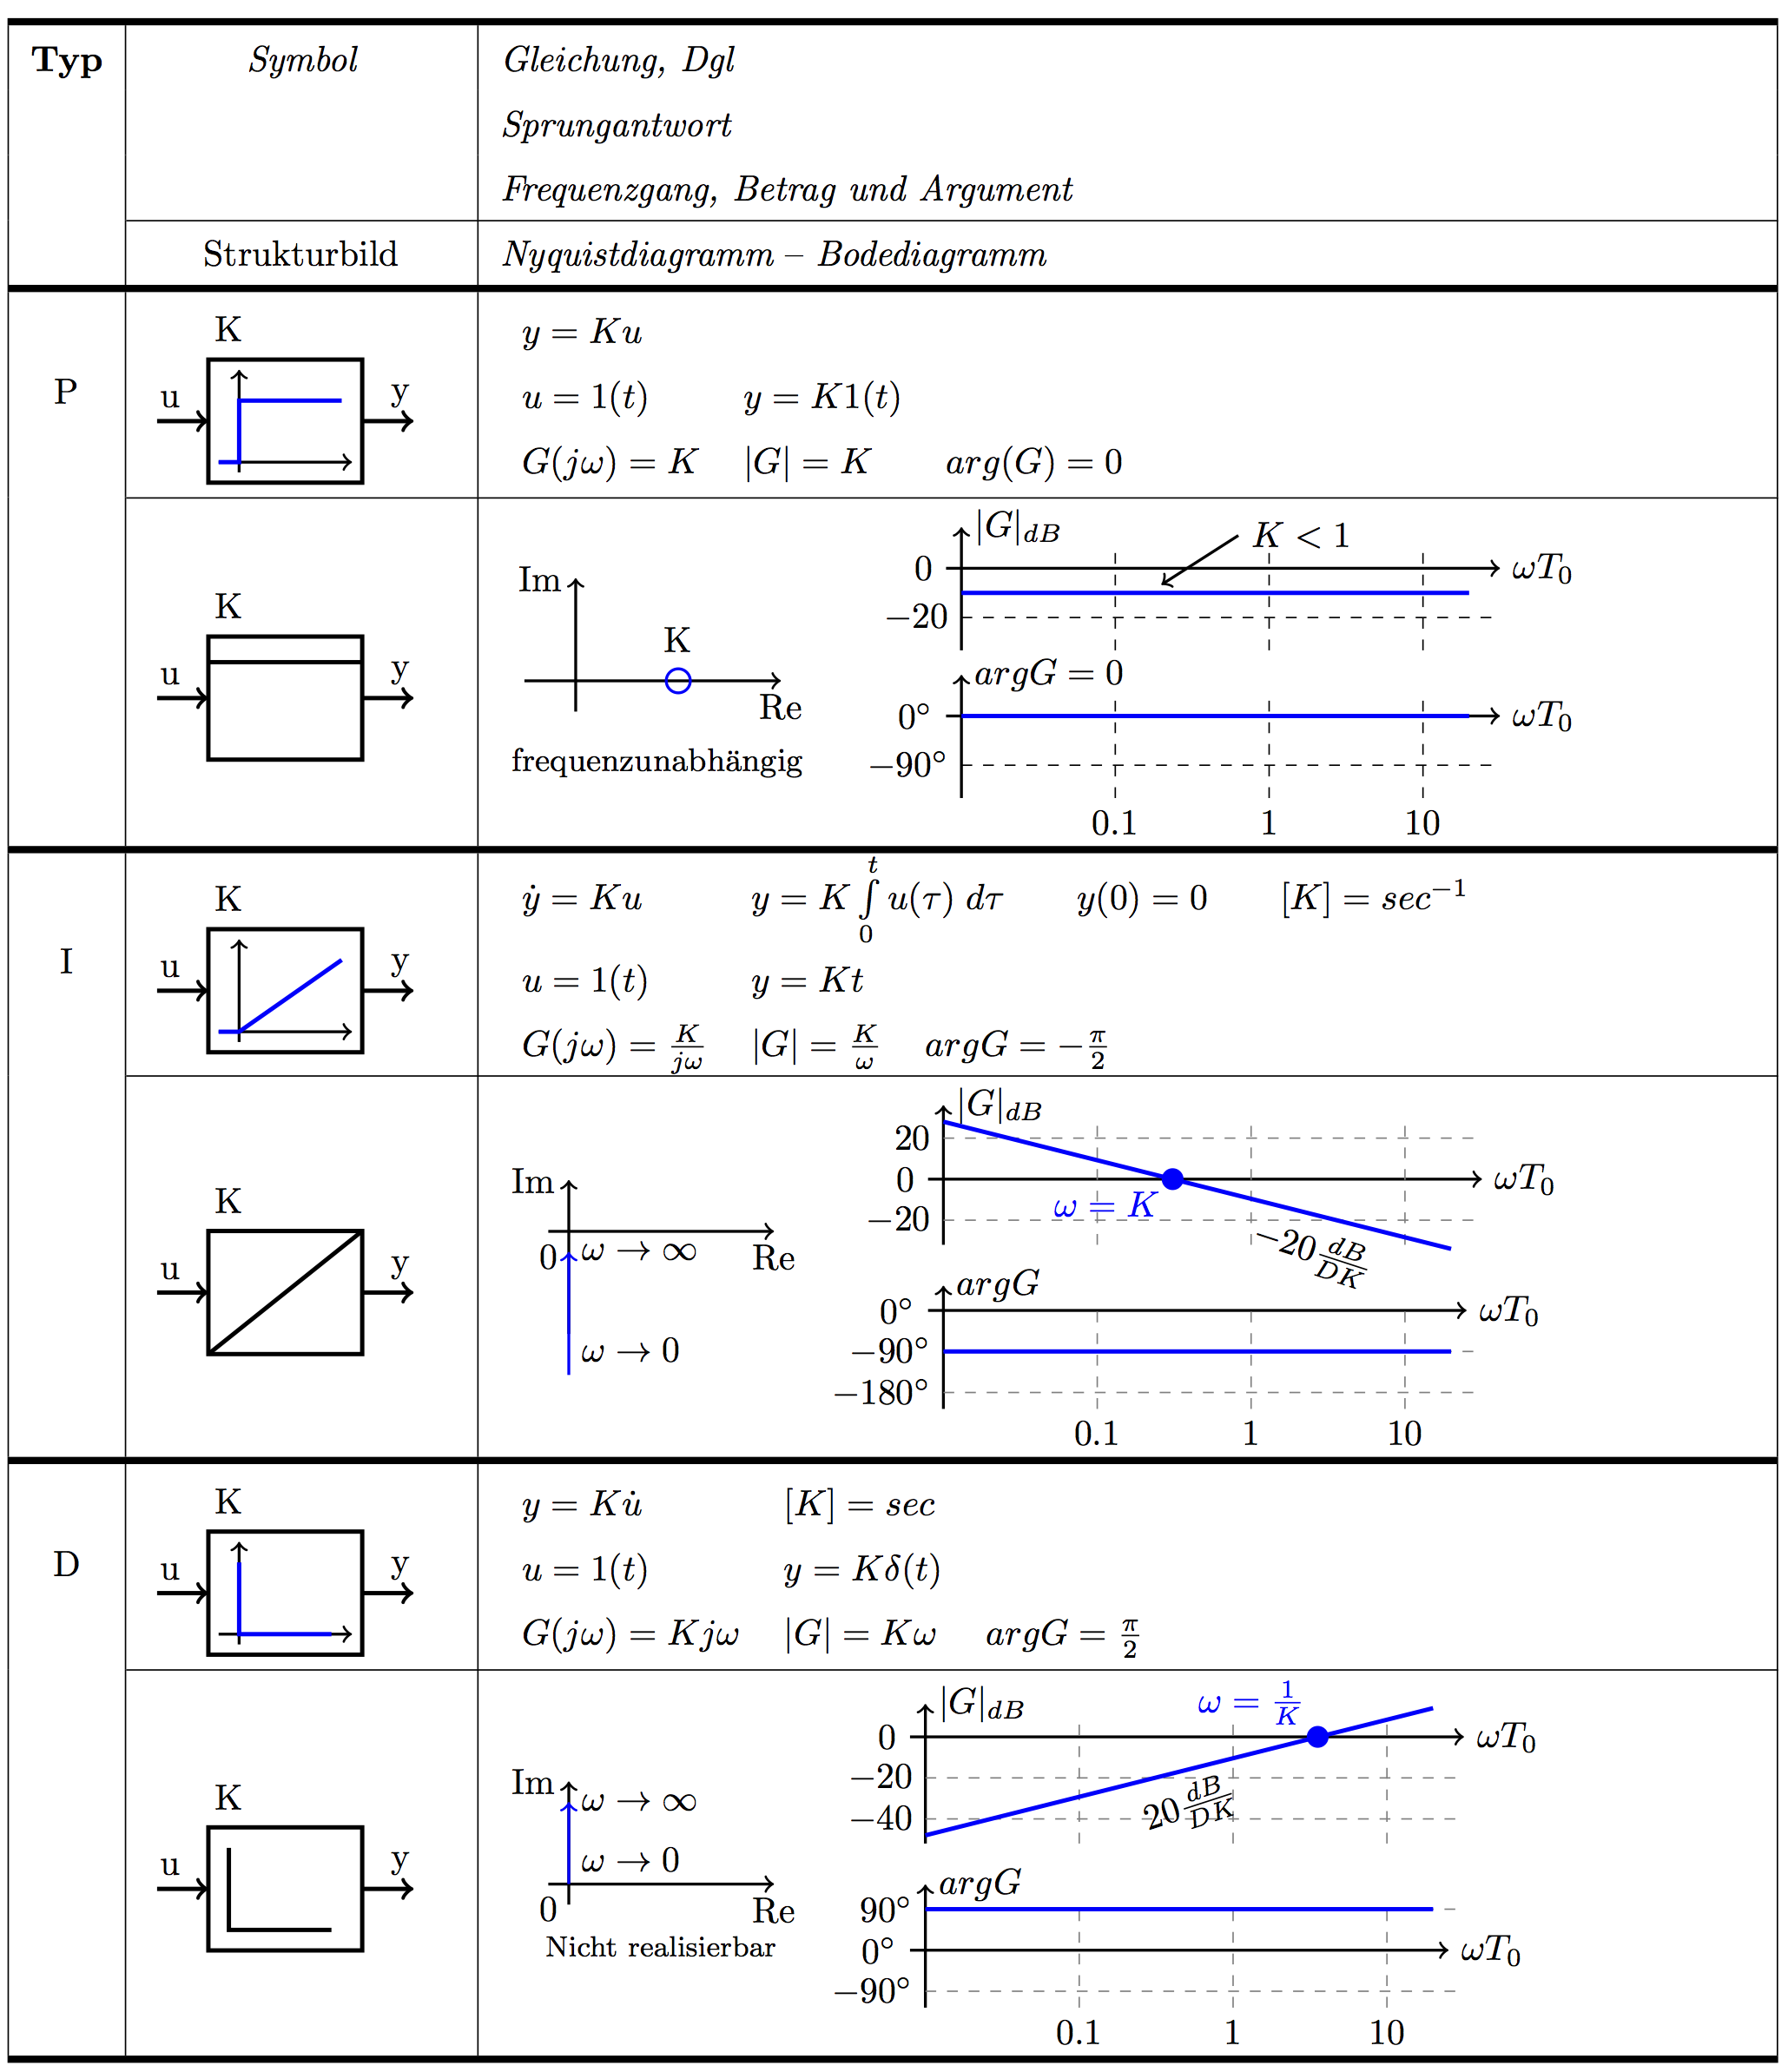
\includegraphics[width=16cm]{./images/LTIGrundGlieder1.png}
      \clearpage
       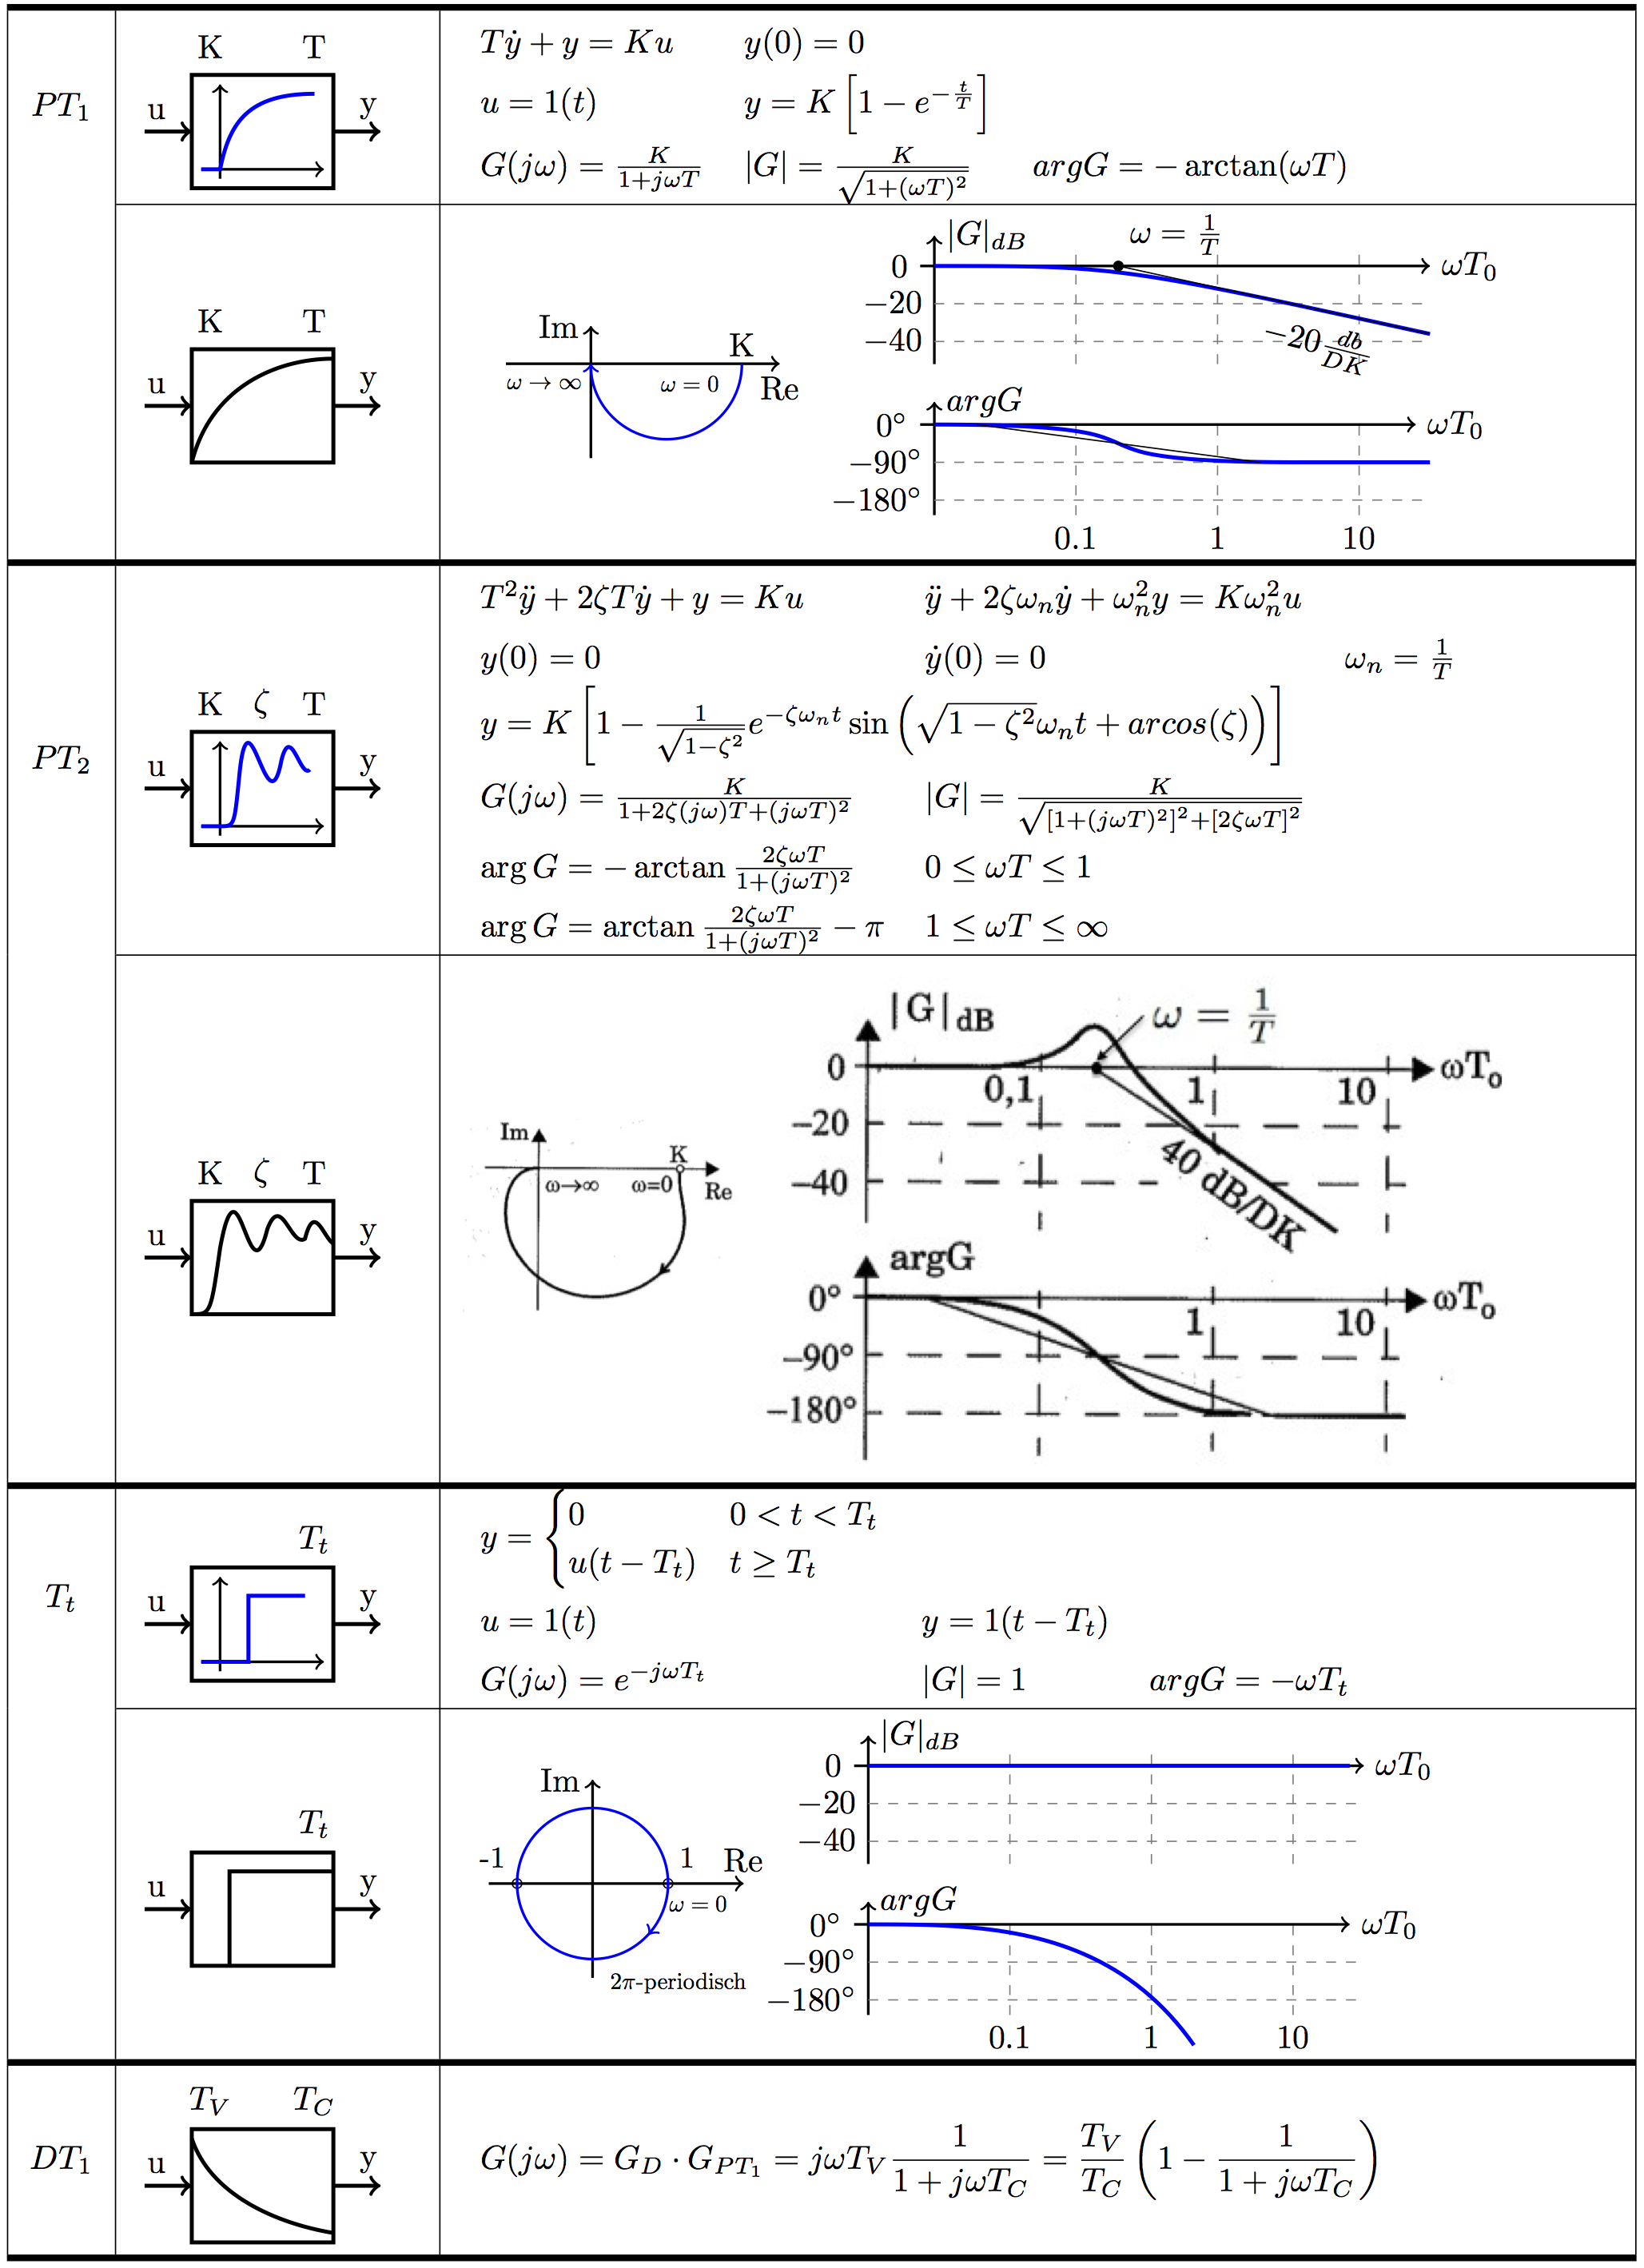
\includegraphics[width=16cm]{./images/LTIGrundGlieder2.png}
    \end{center}
      
  